% ============================================================================
%  Beautified Is Not Forged -- paper v2 (restructured 2026-09-29 around the vendor-supervised model).
%  Every number comes from a results file; tables are generated by make_tables*.py, figures by make_*.py.
%  Moved material lives in supplement.tex. Previous versions: main_pre_8page_20260930.tex, main_pre_restructure_20260929.tex.
% ============================================================================
\documentclass[conference]{IEEEtran}
\IEEEoverridecommandlockouts
\usepackage{fontspec}
\setmainfont{texgyretermes}[Extension=.otf,UprightFont=*-regular,BoldFont=*-bold,ItalicFont=*-italic,BoldItalicFont=*-bolditalic]   % Times: IEEEtran asks for ptm, which XeTeX/tectonic cannot load (bold/italic were silently lost)
\usepackage{cite}
\usepackage{amsmath,amssymb,amsfonts}
\usepackage{graphicx}
\usepackage{booktabs}
\usepackage{adjustbox}
\usepackage{xcolor}
\usepackage{url}
\usepackage{capt-of}
\usepackage{algorithm}
\usepackage{algpseudocode}
\usepackage[hidelinks]{hyperref}
\graphicspath{{figs/}}
\newcommand{\ours}{\textsc{Ours}}
\newcommand{\pending}[1]{\textcolor{orange}{[#1]}}
\renewcommand{\dbltopfraction}{0.92}
\renewcommand{\topfraction}{0.92}
\raggedbottom

\begin{document}

\title{Beautified Is Not Forged:\\Separating Beautification from Face Forgery}

\author{\IEEEauthorblockN{Qin-Ying Lin, Bo-Rong Chen, Chen-Shan Yu}}

\IEEEaftertitletext{\vspace{-0.6\baselineskip}\begin{center}
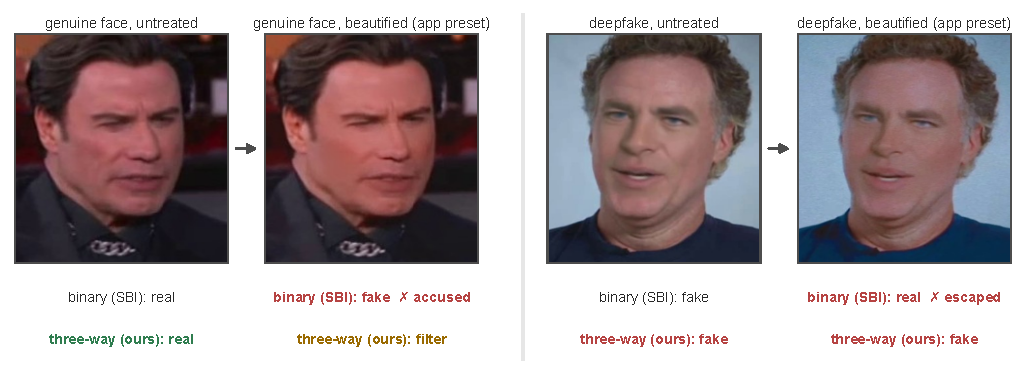
\includegraphics[width=0.92\textwidth]{fig_teaser}
\captionof{figure}{Celeb-DF-B frames of a genuine video and of a deepfake, before and after the same app beautification.
The official SBI checkpoint, at its 5\%-FPR threshold on untreated genuine frames, accuses the beautified genuine face and
lets the beautified deepfake pass. \ours{} calls the first \emph{filter} and the second \emph{fake}. Frames were chosen
where SBI errs after beautification; rates over the benchmark are in Table~\ref{tab:main}.}\label{fig:teaser}
\end{center}\vspace{0.2\baselineskip}}
\maketitle

\begin{abstract}
Face-forgery detectors decide between real and fake, while many genuine faces have been beautified by a camera app or a
retouching service. We measure what this does to thirteen published detectors, including two CLIP-based detectors from
2025. When genuine and forged FaceForensics++ frames receive the same beautification, keeping the escape of beautified
forgeries under 5\% makes every detector accuse at least 14.5\% of beautified genuine faces. On Celeb-DF-B, app beautification raises the share of
deepfakes called real by 3.4 to 35.5 percentage points for the eleven detectors that detect its deepfakes above chance.
A third class, \emph{filter}, for identity-preserving edits removes this effect when everything else in training is
held fixed. A filter class learnt from scripted operations, however, does not recognise commercial retouching:
FF++-trained models separate retouched from untouched faces at chance. We train the three-way detector on the renders of
two commercial retouching services, split by optical flow and frequency into single-operation components with exact
edit footprints, and test it on a third service. A CLIP ViT-L/14 model with LoRA trained this way calls 0.1\% of the
unseen service's retouched faces fake, matches Effort and Forensics Adapter on Celeb-DF-v2 and DFD (video-level AUC 0.954
and 0.983), and is not affected by beautification once re-encoding is accounted for. Its evidence head names regions
whose restoration removes 91\% of its detections on held-out part-level forgeries. Telling the service's lightly
retouched faces from their originals remains difficult (70\% balanced accuracy).
\end{abstract}

% ----------------------------------------------------------------------------
\section{Introduction}
Skin smoothing, whitening, eye enlargement and face slimming are default options in camera apps and are sold as services
by retouching APIs, so many of the genuine faces a detector sees have been edited. Face-forgery detectors are
trained to separate genuine from manipulated faces, and beautification manipulates pixels without changing who is in
the picture. Libourel et al.~\cite{libourel2024} released Celeb-DF-B, a beautified version of Celeb-DF, measured drops of
0.15--0.16 in the video-level AUC of three detectors, and concluded that ``the use of a dedicated filter detection method
is strongly advisable''. Saeed et al.~\cite{saeed2025} show that enhancement lets deepfakes evade detectors, and Concas
et al.~\cite{concas2025} that beauty filters raise the error of deepfake and morphing-attack detectors.

In a binary label space a beautified genuine face has to be called real or fake. Calling it fake is a false accusation.
Calling it real teaches the detector that beautification is a sign of authenticity, and a beautified deepfake then passes
as real (Fig.~\ref{fig:teaser}). A single threshold trades the two errors against each other. We sweep that threshold for thirteen published
detectors and study a third label, \emph{filter}, for edits that keep the identity.

The third label does not suffice by itself. Detectors trained on FaceForensics++ (FF++)~\cite{ffpp} call blurred genuine
faces fake, and a filter class trained on hand-written beautification scripts misses the retouching of commercial services.
Renders of commercial services would teach it, but they apply several operations at once, and a model trained on them
learns which operations co-occur. We therefore split each render into single-operation components that are pixel-aligned
with the original, which gives both a label and an exact footprint for every edit.

Our contributions are:
\begin{itemize}
\item \textbf{A measurement of the problem.} Threshold sweeps of thirteen detectors on a paired FF++ corpus and on
Celeb-DF-B, a same-pipeline replication that isolates the label space, and 2,210 before/after pairs from a commercial
service as a test of retouching recognition.
\item \textbf{Supervision from commercial renders.} A decomposition of multi-operation renders into single-operation
components (Alg.~\ref{alg:decomp}), used with degradation applied equally to all classes and with part-level forgeries
to train one three-way detector.
\item \textbf{Evidence with a faithfulness test.} An evidence head trained on exact edit footprints, and a restoration
test that checks whether the region it names is sufficient and necessary for the decision.
\end{itemize}
The three-class formulation itself is not new. ForgeryNet~\cite{forgerynet} has a three-way task in which
identity-preserving edits count as forgeries, and Bobulski and Kubanek~\cite{bobulski2024} classify real, photo-edited
and generated faces. We assign beautification to a genuine outcome and train with commercial renders.

% ----------------------------------------------------------------------------
\section{Related Work}
\textbf{Beautification and forgery detection.} The studies cited in the introduction~\cite{libourel2024,saeed2025,concas2025}
evaluate existing detectors; none of them trains a detector that removes the effect.

\textbf{Retouching detection.} RetouchingFFHQ~\cite{retouchingffhq} labels four commercial operations at three levels and
reports cross-vendor recall. Diffusion models restore the untouched face~\cite{frrffusion,mofrr}, a level classifier can
guide the reversal~\cite{reface}, and predicted warp fields undo Photoshop liquify~\cite{wang2019photoshop}. These methods
have no forgery class.

\textbf{Generalisable forgery detection.} Face X-ray~\cite{facexray} and SBI~\cite{sbi} synthesise blending artefacts
from real images, and UCF~\cite{ucf} separates common forgery features from content and method-specific ones.
Effort~\cite{effort} and Forensics Adapter~\cite{forensicsadapter} adapt CLIP ViT-L/14 with few trainable parameters and
report the strongest cross-dataset results of recent work. DeepfakeBench~\cite{deepfakebench} provides common
checkpoints for many detectors.

\textbf{Explanations for detectors.} GAIN~\cite{gain} trains attention maps so that erasing the attended region removes
the class evidence, amortised maskers predict saliency in one pass~\cite{dabkowski2017,phang2020}, and DOLOS~\cite{dolos}
compares explanation, local-score and attention methods for localising inpainted face regions and finds local scores
best. We supervise the map with exact footprints and test it by restoring pixels.

% ----------------------------------------------------------------------------
\begin{figure*}[t]
\centering
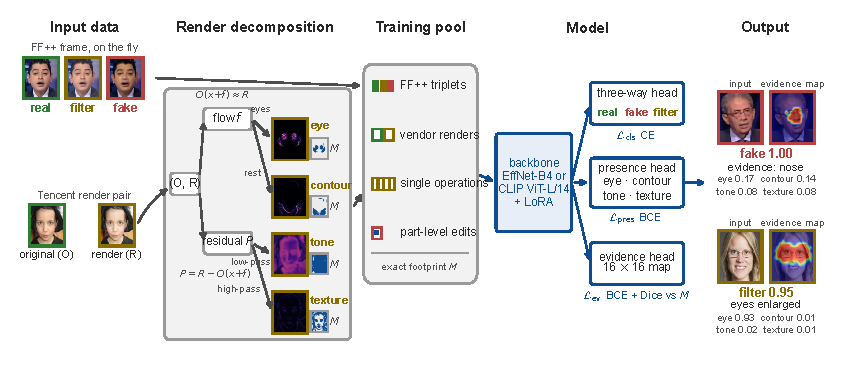
\includegraphics[width=\textwidth]{fig_overview}
\caption{Overview. Each genuine FF++ photograph yields a real / filter / fake triplet on the fly; a beautified forgery
stays \emph{fake}. Each commercial render $R$ of an original $O$ is split by its optical flow $f$ and photometric residual
$P$ into four single-operation components (shown as $|\text{component}-O|$), each with an exact footprint $M$
(Eq.~\ref{eq:footprint}, Alg.~\ref{alg:decomp}). One backbone feeds a three-way head, an operation-presence head and an
evidence head trained against $M$ (Eq.~\ref{eq:loss}). Right: outputs of \ours{} on a held-out part-level forgery and on a
render from the unseen service.}
\label{fig:pipeline}
\end{figure*}

\section{Method}
\label{sec:method}
\subsection{Labels and errors}
The label of a face $x$ is $y\in\{\textsc{real},\textsc{fake},\textsc{filter}\}$. \textsc{real} is an unedited photograph,
\textsc{fake} covers identity swap, reenactment and synthesis, and \textsc{filter} covers edits that keep the identity
(smoothing, whitening, eye enlargement, face slimming, colour grading). A face that was forged and then beautified is
\textsc{fake}. The detector outputs class probabilities $p(x)$, presence scores $\hat s(x)\in[0,1]^4$ for eye, contour,
tone and texture edits, and an evidence map $\hat m(x)$. The decision is $\hat y=\arg\max_c p_c(x)$.

Two error rates describe beautification. FA is the share of beautified genuine faces with $\hat y=\textsc{fake}$ and
MISS the share of beautified forgeries with $\hat y=\textsc{real}$; a beautified forgery sent to \textsc{filter} counts
in neither. A binary detector with score $s$ traces a curve $(\mathrm{FA}(t),\mathrm{MISS}(t))$ over thresholds $t$ and
\emph{dominates} a three-way detector with errors $(\mathrm{FA}^*,\mathrm{MISS}^*)$ if some $t$ gives
$\mathrm{FA}(t)\le\mathrm{FA}^*$ and $\mathrm{MISS}(t)\le\mathrm{MISS}^*$. We sweep every threshold on the test set, which
favours the binary detectors.

\subsection{Supervision from paired originals}
Every edited image $x$ in our training pool has a pixel-aligned original $x_0$, and the pair defines where the edit is:
\begin{equation}
M(x)=\mathrm{dilate}_\rho\!\big(\mathbf{1}[\,\|x-x_0\|_\infty>\tau\,]\big),
\label{eq:footprint}
\end{equation}
with $\tau=6$ on 8-bit intensities and $\rho$ the feather width of the edit. Observed FF++ forgeries have no aligned
original and get no footprint. The pool has four sources (Fig.~\ref{fig:pipeline}).

\textbf{FF++ triplets.} FF++ c23 under the official 720/140/140 video split. For each genuine training photograph $x_0$
a step draws a \textsc{real} item ($x_0$), a \textsc{filter} item (an on-the-fly beautification of $x_0$ by one of four
landmark and skin operations at a random strength or by one of 14 photometric filters~\cite{pilgram}, otherwise an
observed filter frame) and a \textsc{fake} item (a self-blend of $x_0$~\cite{sbi}, an observed forgery from the four FF++
methods, or a part-level forgery). A fake is beautified on top with probability 0.5. The same random blur or downscale is
applied to all three items, so that sharpness does not predict the class.

\textbf{Commercial renders.} 7,831 FFHQ photographs~\cite{ffhq} (indices 60002--69999) enter \textsc{real} and serve as
self-blend bases, so that a clean still photograph is not a class cue. Their renders by two retouching APIs from
RetouchingFFHQ~\cite{retouchingffhq}, Tencent (7,730 renders at levels 30/60/90) and Megvii (13,139), enter
\textsc{filter}. Both services apply eye enlargement, face lifting, whitening and smoothing together, and a model
trained on the renders learns to rely on the texture change (Sec.~\ref{sec:ali}). We split each render $R$ of an original
$O$ into single-operation components in $O$'s geometry (Alg.~\ref{alg:decomp}). Dense optical flow~\cite{dis} on locally
normalised luminance gives $f$ with $O(\mathbf{u}+f(\mathbf{u}))\approx R(\mathbf{u})$, and the photometric residual in
$O$'s geometry is
\begin{equation}
P(\mathbf{u})=R\big(\mathbf{u}-f^{-1}(\mathbf{u})\big)-O(\mathbf{u}).
\label{eq:residual}
\end{equation}
With $E$ the eye-region mask, $\mathcal{W}(O;g)$ the warp of $O$ by a flow $g$ and $G_\sigma$ a Gaussian ($\sigma=6$\,px
at 512\,px), the components are
\begin{align}
C_\text{eye} &= \mathcal{W}(O;\,E\odot f), & C_\text{contour} &= \mathcal{W}(O;\,(1-E)\odot f), \nonumber\\
C_\text{tone} &= O + G_\sigma * P, & C_\text{texture} &= O + P - G_\sigma * P.
\label{eq:components}
\end{align}
Applying the four edits in sequence reproduces $R$ at 108\,dB PSNR. Each component is a \textsc{filter} item whose
presence target is its operation. Components whose measured edit (below) falls under the noise floor of the measurement
are dropped, leaving 50,112 of 73,952. Parametric single operations, with strengths drawn log-uniformly from the range
measured on the two services, complete the filter pool. The third service, Alibaba (FFHQ indices 17001--19999, one
operation per render), is used only for testing, and the content keys of its 28,729 images and of the 7,831 training
bases are disjoint.

\begin{algorithm}[t]
\caption{Single-operation components of a commercial render}
\label{alg:decomp}
\begin{algorithmic}[1]
\Require original $O$, render $R$, eye mask $E$, $\sigma$, noise floors $\tau_k$
\State $f\gets\mathrm{DIS}\big(\mathrm{LCN}(O),\mathrm{LCN}(R)\big)$ \Comment{normalised luminance}
\State $P\gets R\circ(\mathrm{id}-f^{-1}) - O$ \Comment{Eq.~\ref{eq:residual}}
\State $C_\text{eye}\gets\mathcal{W}(O;E\odot f)$;\quad $C_\text{contour}\gets\mathcal{W}(O;(1-E)\odot f)$
\State $C_\text{tone}\gets O+G_\sigma*P$;\quad $C_\text{texture}\gets O+P-G_\sigma*P$
\For{$k\in\{\text{eye},\text{contour},\text{tone},\text{texture}\}$}
  \State $q_k\gets\mathrm{Measure}_k(C_k,O)$
  \If{$q_k\ge\tau_k$} \State keep $(C_k,\ e_k,\ M(C_k))$ \Comment{Eq.~\ref{eq:footprint}} \EndIf
\EndFor
\end{algorithmic}
\end{algorithm}

\textbf{Part-level forgeries.} We build 61,510 training forgeries and a held-out test set on FF++ frames by transplanting
the eyes, nose or mouth of another identity (landmark-aligned warp, colour matching, feathering) or by regenerating the
part with Stable Diffusion 1.5 inpainting. Pixels outside the feathered mask are copied bit-exactly from $x_0$, so
Eq.~\ref{eq:footprint} is exact. SDXL inpainting is generated for test frames only.

\textbf{Edit measurements.} For each aligned pair we measure $q=(r_\text{eye}-1,\ 1-r_\text{jaw},\ \Delta L/20,\
1-r_\text{hf})$, the eye- and jaw-width ratios from re-detected landmarks, the CIELAB lightness change and the
high-frequency energy ratio inside the face hull. The measurements set the noise floors $\tau_k$. A head that regressed
$q$ did not pass validation (supplement).

\subsection{Model and objective}
A backbone $\phi$ feeds three heads. For \ours{} it is a frozen CLIP ViT-L/14~\cite{clip} with rank-16 LoRA~\cite{lora}
on every attention projection (3.2\,M trained parameters of 306\,M); for \ours{}-lite it is EfficientNet-B4~\cite{efficientnet}
(17.6\,M). The three-way head and the presence head read the pooled feature, and the evidence head
$\hat m=\sigma(g(\phi_\text{sp}(x)))$ is a $1\times1$ convolution on the spatial tokens ($16\times16$ for CLIP, $12\times12$
for EfficientNet-B4). The loss on one item is
\begin{align}
\mathcal{L}={}&\mathrm{CE}(p,y)+\lambda_s\,\mathbf{1}[y=\textsc{filter}]\,\mathrm{BCE}(\hat s,s) \nonumber\\
&+\lambda_m\,\mathbf{1}[M\ \text{exact}]\,\big(\mathrm{BCE}(\hat m,M)+\mathrm{Dice}(\hat m,M)\big),
\label{eq:loss}
\end{align}
with $\lambda_s=\lambda_m=1$. Real items have an empty footprint and observed forgeries no footprint term. The
classifier does not read $\hat m$, so whether the map explains the decision has to be tested.

\textbf{Faithfulness test.} For a detected part-level forgery with footprint $M$, let $\hat A$ be the $|M|$ highest cells of
$\hat m$, dilated by the feather width, and let $x_A=x\odot(1-A)+x_0\odot A$ restore a region $A$ to the original. We
report the flip rate $\Pr[\arg\max p(x_{\hat A})\neq\textsc{fake}]$ and the same rate for the complement $1-\hat A$, for
the true footprint $M$ (the ceiling), for a centred region and for a random region of equal area, together with the IoU of
$\hat m$ and $M$ on a $7\times7$ grid (IoU$_7$). A faithful map flips as often as the true footprint and its complement
does not flip.

\textbf{Training.} CLIP: 224\,px, AdamW at $10^{-4}$ with warm-up and cosine decay, 8 epochs. EfficientNet-B4 (AdvProp
weights~\cite{advprop}): 380\,px, SGD at $10^{-3}$ with SAM~\cite{sam}, 12 epochs. A batch holds 16 genuine bases (48
items); fakes are drawn as self-blends (0.4), observed forgeries (0.3) or part-level forgeries (0.3). Checkpoints are
selected on FF++ validation macro-F1 plus F1 on held-out Tencent and Megvii bases. No cross-dataset set is used for any
choice.

% ----------------------------------------------------------------------------
\section{Experimental Setup}
\label{sec:protocol}
\textbf{Test sets.} FF++ c23 test (1,316 real, 5,304 fake and 1,316 filter frames) with 400 test forgeries under eight
beautification conditions; Celeb-DF-v2~\cite{celebdf} (official list, 518 videos, 16,059 frames); DFD~\cite{dfd} (332
held-out videos, 4,221 frames); Celeb-DF-B in the release provided by its authors, with 232 genuine and 232 synthesis
videos, each untreated, beautified by one of four app presets and re-encoded without a filter (43,363 frames); and the
Alibaba pairs (2,210 FFHQ originals, 26,519 renders, four operations at three levels). Video sets use 32 evenly spaced
frames per video.

\textbf{Metrics.} Frame-level AUC and video-level AUC (mean of the 32 frame scores), with 95\% video-cluster bootstrap
intervals; model differences use a paired bootstrap on the same frames. For commercial retouching, balanced accuracy
averages the share of renders called \textsc{filter} and the share of originals not called \textsc{filter}.

\textbf{Baselines.} Thirteen detectors with their released weights: eight DeepfakeBench checkpoints (Xception,
EfficientNet-B4, F3Net, SPSL, UCF, RECCE, CORE, SRM), the official SBI, Effort and Forensics Adapter, UnivFD~\cite{univfd}
and NPR~\cite{npr}. All are scored on our frames with our crops. For Xception, EfficientNet-B4 and UCF, whose frame-level Celeb-DF-v2
AUCs are published for this protocol, our scores are within 0.02 of them (supplement).

\textbf{Protocol.} Target values for every model were written down before training and are reported whether met or not.
Each model reads the Alibaba set once.

% ----------------------------------------------------------------------------
\begin{table*}[t]
\centering
\caption{Forgery detection and beautification errors on the same frames. AUC of $P(\text{fake})$ at frame and video level;
Celeb-DF-B AUC on untreated genuine vs.\ synthesis frames. FA: beautified genuine faces called fake, MISS: beautified
forgeries called real (\%). For binary detectors the FA is the lowest one a threshold on the test set reaches while
keeping MISS at the stated level; $\Delta$MISS is the change caused by Celeb-DF-B beautification at 5\% FPR on untreated
genuine frames. Three-way models use no threshold. Bold: best per column; $\Delta$MISS is not marked because its
smallest values belong to detectors that barely detect Celeb-DF-B deepfakes (UnivFD, NPR).}
\label{tab:main}
\footnotesize
\begin{adjustbox}{max width=\textwidth}\begin{tabular}{lr cc cc c c cc}
\toprule
 & & \multicolumn{2}{c}{Celeb-DF-v2} & \multicolumn{2}{c}{DFD} & Celeb-DF-B & FF++ beautified & \multicolumn{2}{c}{Celeb-DF-B beautified} \\
\cmidrule(lr){3-4}\cmidrule(lr){5-6}\cmidrule(lr){7-7}\cmidrule(lr){8-8}\cmidrule(lr){9-10}
Detector & Params (M) & frame & video & frame & video & AUC & FA at MISS$\le$5 & $\Delta$MISS & FA at MISS$\le$9.7 \\
\midrule
\multicolumn{10}{l}{\textit{Published binary detectors, official weights, our frames; FA read off the full threshold sweep}} \\
Xception & 21.9 & 0.718 & 0.772 & 0.897 & 0.882 & 0.811 & 19.1 & +9.9 & 65.7 \\
EfficientNet-B4 & 19.3 & 0.750 & 0.807 & 0.862 & 0.860 & 0.811 & 19.2 & +3.4 & 59.2 \\
F3Net & 21.9 & 0.708 & 0.750 & 0.852 & 0.811 & 0.798 & 14.5 & +6.8 & 66.1 \\
SPSL & 21.9 & 0.703 & 0.752 & 0.873 & 0.851 & 0.781 & 19.9 & +13.1 & 63.3 \\
UCF & 21.9 & 0.744 & 0.788 & 0.877 & 0.853 & 0.841 & 16.1 & +12.4 & 59.6 \\
RECCE & 47.7 & 0.688 & 0.731 & 0.900 & 0.877 & 0.785 & 22.6 & +11.8 & 68.2 \\
CORE & 21.9 & 0.715 & 0.764 & 0.882 & 0.859 & 0.821 & 19.1 & +13.8 & 63.4 \\
SRM & 53.2 & 0.717 & 0.778 & 0.893 & 0.869 & 0.789 & 19.1 & +17.0 & 65.4 \\
SBI & 17.6 & 0.817 & 0.872 & 0.918 & 0.876 & 0.875 & 40.4 & +35.5 & 67.3 \\
Effort (CLIP-L/14) & 303.4 & 0.881 & 0.930 & 0.935 & 0.957 & 0.909 & 36.5 & +23.7 & 61.2 \\
Forensics Adapter (CLIP-L/14) & 309.7 & 0.887 & 0.945 & 0.942 & 0.959 & 0.909 & 30.5 & +15.5 & 53.6 \\
UnivFD & 427.6 & -- & -- & -- & -- & 0.653 & 80.2 & $-$0.2 & 81.7 \\
NPR & 1.4 & -- & -- & -- & -- & 0.503 & 92.4 & +1.6 & 90.5 \\
\midrule
\multicolumn{10}{l}{\textit{Three-way, native argmax rule, no threshold (MISS in parentheses)}} \\
\textbf{\ours{}} (CLIP ViT-L/14 + LoRA) & 306.3 & \textbf{0.888} & \textbf{0.954} & \textbf{0.948} & \textbf{0.983} & \textbf{0.937} & \textbf{4.0} (0.6) & +2.9 & \textbf{18.4} (9.7) \\
\ours{}-lite (EfficientNet-B4) & 17.6 & 0.848 & 0.910 & 0.915 & 0.908 & 0.899 & 11.7 (0.5) & +3.9 & 21.9 (7.3) \\
\bottomrule
\end{tabular}
\end{adjustbox}
\end{table*}

\begin{figure*}[t]
\centering
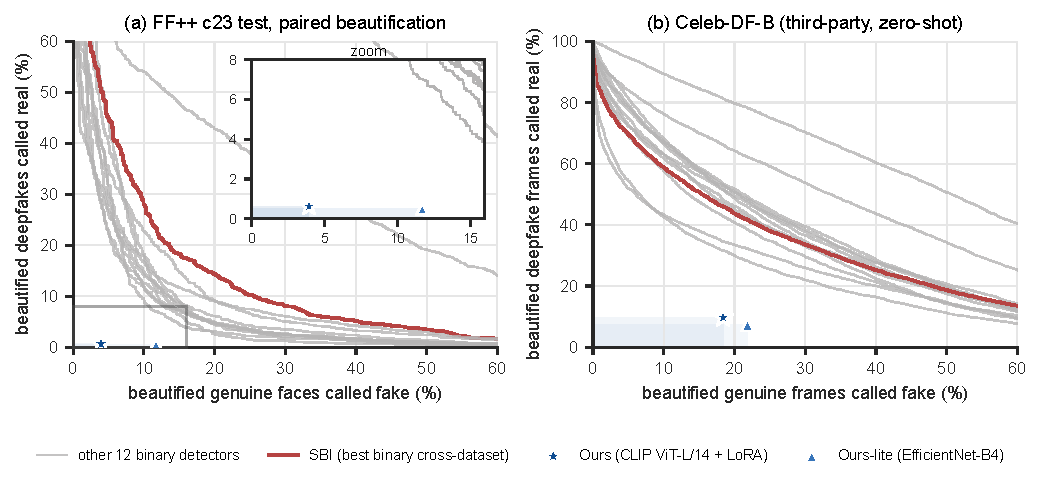
\includegraphics[width=0.8\textwidth]{fig_frontier}
\caption{Threshold sweeps. Each grey curve is one published detector over all thresholds, SBI in red. Markers are the
three-way models at their native rule; the shaded box under a marker is where a binary detector would have to reach to
dominate it. (a) FF++ c23 test, beautification applied to the same frames. (b) Celeb-DF-B, app beautification. No curve
enters a box.}
\label{fig:frontier}
\end{figure*}

\section{Results}
\label{sec:results}
\subsection{Threshold sweeps}
On the FF++ corpus, keeping MISS at or below 5\% makes the published detectors accuse between 14.5\% (F3Net) and 92.4\%
(NPR) of beautified genuine faces (Table~\ref{tab:main}, Fig.~\ref{fig:frontier}). \ours{} accuses 4.0\% and misses
0.6\% with no threshold. On Celeb-DF-B, reaching our MISS of 9.7\% costs the binary detectors an FA of 53.6--90.5\%,
against 18.4\% for \ours{}. No threshold of any published detector dominates \ours{} or \ours{}-lite on either benchmark,
and the same holds for every three-way variant in the supplement that saw real forgeries in training. The variant whose
fake class contains only self-blends is dominated by six of twelve detectors on FF++.

\subsection{Escape under beautification}
We fix each binary detector at 5\% FPR on untreated Celeb-DF-B genuine frames and compare the share of deepfakes called
real before and after beautification ($\Delta$MISS in Table~\ref{tab:main}). The share rises by 3.4 to 35.5\,pp for the
eleven detectors that separate untreated Celeb-DF-B deepfakes above chance, all with intervals above zero: SBI from
44.3\% to 79.8\%, Effort from 27.8\% to 51.4\%, Forensics Adapter from 31.1\% to 46.5\%. UnivFD and NPR move by less than
2\,pp, but their untreated AUC is 0.65 and 0.50. Celeb-DF-B re-encodes every treated video, and its compression-only
videos separate the two causes. Re-encoding alone raises the escape of SBI by 13.7\,pp, leaving 21.8\,pp for
beautification; the remainder is 11.0\,pp for Effort and 15.3\,pp for Forensics Adapter. \ours{} rises by 2.9\,pp
overall and by 3.4\,pp under re-encoding alone, so beautification adds nothing measurable; \ours{}-lite adds 0.9\,pp.
\ours{} sends 36.9\% of beautified genuine frames to \textsc{filter}. Its largest per-preset change is +7.4\,pp for the
warm colour grade \emph{california\_dreamin} (supplement).

To separate the label space from the rest of the pipeline, we retrained SBI's binary objective with the backbone, recipe,
data and frames of our FF++-only three-way model. Its escape rises by 36.8\,pp [33.2, 40.8], close to the 35.5\,pp of the
official SBI, while the three-way model trained with the same blending changes by 0.1\,pp [$-$1.3, 1.7].

\subsection{Blur}
On 300 genuine FF++ test frames, a Gaussian blur with $\sigma=1.5$ makes SBI call 67\% of them fake, Xception 53\%,
EfficientNet-B4 57\% and UCF 42\%, and our FF++-only three-way model 91--95\%. JPEG compression at quality 30 changes
none of these by more than 5\,pp. Self-blending softens one side of the blend, and a detector trained on it learns that a
soft face is a forged one. Celeb-DF genuine frames are softer than FF++ frames at the same crop size, and the FF++-only
model calls 43--51\% of untreated Celeb-DF-B genuine frames fake. Degrading the three items of a triplet together reduces
blurred genuine frames called fake to 10\% and the untreated Celeb-DF-B accusation to 28\%. \ours{} calls 16.9\% of
untreated Celeb-DF-B genuine frames fake and \ours{}-lite 40.3\%.

\subsection{Commercial retouching}
\label{sec:ali}
\begin{table*}[t]
\centering
\caption{Retouching by a service never seen in training: 2,210 FFHQ originals and their Alibaba renders (four operations
at three levels, 26,519 images). Paired rank: share of pairs in which the render gets a higher $P(\text{filter})$ than its
own original (50 means no signal). Native argmax rule. All other variants are in the supplement.}
\label{tab:alipair}
\footnotesize
\begin{adjustbox}{max width=\textwidth}\begin{tabular}{l c cc c c c c}
\toprule
 & originals & \multicolumn{2}{c}{retouched (pooled)} & & & paired rank at level 90 & smoothing-90 \\
\cmidrule(lr){3-4}
Model & real/fake/filter & $\to$filter & $\to$fake & balanced & paired rank & eye / white / lift / smooth & $\to$fake \\
\midrule
\multicolumn{8}{l}{\textit{FF++ c23 training only (zero-shot)}} \\
three-way, observed fakes (SUP) & 36.8/5.7/57.5 & 66.5 & 9.1 & 54.5 & 79.8 & 97 / 89 / 79 / 59 & 27.3 \\
three-way, part edits + evidence head & 16.7/55.9/27.4 & 28.6 & 59.4 & 50.6 & 60.9 & 89 / 78 / 60 / 20 & 85.8 \\
\midrule
\multicolumn{8}{l}{\textit{Trained with two vendors' renders and their single-operation components; Alibaba never seen (ours)}} \\
\textbf{\ours{}} (CLIP ViT-L/14 + LoRA) & 57.9/0.3/41.9 & 82.3 & 0.1 & 70.2 & 94.8 & 98 / 94 / 95 / 100 & 0.0 \\
\ours{}-lite (EfficientNet-B4) & 81.0/0.4/18.6 & 63.8 & 0.3 & 72.6 & 93.8 & 99 / 91 / 93 / 99 & 0.4 \\
\bottomrule
\end{tabular}
\end{adjustbox}
\end{table*}
\begin{figure}[t]
\centering
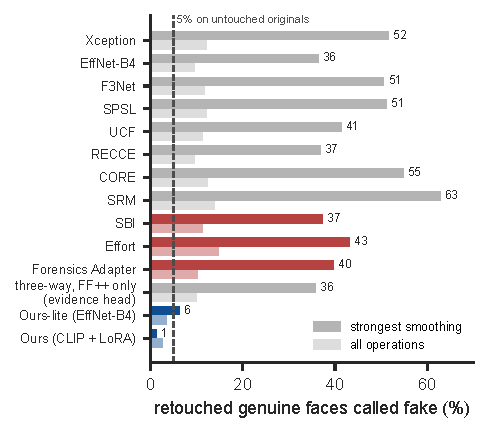
\includegraphics[width=\columnwidth]{fig_accuse}
\caption{Retouched genuine faces from the unseen service called \emph{fake}, each detector at the threshold that calls 5\%
of the untouched originals fake (chosen on the test originals, which favours the binary detectors). Dark: strongest
smoothing; light: all operations and levels. Red: SBI and the two CLIP-based detectors.}
\label{fig:accuse}
\end{figure}
Table~\ref{tab:alipair} and Fig.~\ref{fig:accuse} use the Alibaba service, which applies one operation per render.
Three-way models trained on FF++ alone separate retouched from untouched faces at chance (balanced accuracy 48--55\%
for all six variants). They move originals away from \textsc{real} and call commercial smoothing fake, up to 86\% of
faces at the strongest level. The eleven published detectors trained on FF++ do the same. At a threshold that calls 5\% of the originals fake,
chosen on these originals, they call 9.5--14.8\% of retouched faces and 36--63\% of the most strongly smoothed ones
fake.

\ours{} calls 0.1\% of retouched faces fake, and at the same 5\% threshold 2.7\% of them and 1.4\% of the most strongly
smoothed ones. It sends 82.3\% of retouched faces to \textsc{filter} (levels 30/60/90: eye enlargement 70/79/85\%,
lifting 68/75/80\%, whitening 72/79/85\%, smoothing 96/100/100\%) and gives 94.8\% of renders a higher filter score than
their own original. It also sends 41.9\% of the untouched Alibaba originals to \textsc{filter}, and 44.4\% of the originals held out
from the two training services, so the loss of specificity is not limited to the unseen service; its balanced accuracy
is 70.2\%. \ours{}-lite keeps 81.0\% of the
originals \textsc{real} and reaches 72.6\%. Our target was 75\%. A threshold on $P(\text{filter})$ chosen on the
training services' validation split gives 72.4\%, and the AUROC of $P(\text{filter})$ between originals and renders is
0.80--0.82 for every model trained with components, so no threshold reaches the target. The presence head recalls
smoothing and whitening more often than the Megvii-to-Alibaba numbers reported by RetouchingFFHQ~\cite{retouchingffhq}
(0.96 vs.\ 0.86, 0.57 vs.\ 0.50) and eye enlargement and lifting less often (0.21 vs.\ 0.52, 0.35 vs.\ 0.55), while
marking each operation absent on 82--99\% of originals, which that work does not report.

\subsection{Forgery detection}
Table~\ref{tab:main} lists cross-dataset AUC with every detector scored on the same frames. \ours{} reaches 0.888 at
frame level and 0.954 at video level on Celeb-DF-v2, 0.948 and 0.983 on DFD, and 0.937 on untreated Celeb-DF-B. The
differences to the official SBI checkpoint are positive at both levels on both sets (paired intervals above zero, from
[+0.006, +0.057] for DFD frames to [+0.065, +0.151] for DFD videos). The differences to Effort and Forensics Adapter are
small, and all eight paired intervals contain zero, so we count \ours{} as level with them on these two sets. At 17.6\,M
parameters, \ours{}-lite reaches 0.910 and 0.908 at video level, above SBI on both sets. On the FF++ test split \ours{}
recalls 78.0\% of genuine, 88.9\% of fake and 89.2\% of filter frames; the genuine recall is below the 80\% we targeted,
as are the genuine (74.2\%) and filter (76.4\%) recall of \ours{}-lite.

\subsection{Localisation of part-level forgeries}
\label{sec:cgd}
\begin{table*}[t]
\centering
\caption{Explanations on held-out part-level forgeries (FF++ test frames, detected items only). IoU$_7$: IoU with the
exact footprint on a 7$\times$7 grid. Flip: share of items that leave \emph{fake} when the named region, of the same
area as the footprint, is restored to the original. Ceil.: the same for the true footprint. Compl.: the same for the
complement. SDXL was never used in training. Full table in the supplement.}
\label{tab:cgd_explain}
\footnotesize
\begin{adjustbox}{max width=\textwidth}\begin{tabular}{l cccc cccc cccc}
\toprule
 & \multicolumn{4}{c}{donor transplant} & \multicolumn{4}{c}{SD-1.5 inpaint} & \multicolumn{4}{c}{SDXL inpaint (unseen editor)} \\
\cmidrule(lr){2-5}\cmidrule(lr){6-9}\cmidrule(lr){10-13}
Map & IoU$_7$ & flip & ceil. & compl. & IoU$_7$ & flip & ceil. & compl. & IoU$_7$ & flip & ceil. & compl. \\
\midrule
centre prior / random region (last col.) & 0.310 & 38.6 & -- & 17.0 & 0.249 & 40.9 & -- & 17.9 & 0.255 & 40.2 & -- & 17.7 \\
\midrule
Score-CAM, same backbone, no head & 0.408 & 56.5 & 85.8 & 5.9 & 0.334 & 52.4 & 85.2 & 15.4 & 0.341 & 52.4 & 85.9 & 17.1 \\
head, vendor data, no part edits (CLIP) & 0.479 & 78.8 & 89.4 & 2.5 & 0.376 & 53.9 & 69.1 & 14.4 & 0.445 & 68.9 & 78.3 & 8.4 \\
head, part edits, FF++ only (EffNet-B4) & 0.723 & 84.0 & 84.7 & 0.4 & 0.752 & 82.6 & 83.2 & 0.7 & 0.746 & 82.9 & 83.8 & 0.7 \\
\ours{}-lite (EffNet-B4) & 0.804 & 87.8 & 87.8 & 0.1 & 0.820 & 87.4 & 87.6 & 0.4 & 0.812 & 86.9 & 87.2 & 0.4 \\
\textbf{\ours{}} (CLIP ViT-L/14 + LoRA) & 0.832 & 91.7 & 91.9 & 0.1 & 0.845 & 91.5 & 91.6 & 0.2 & 0.827 & 90.9 & 91.2 & 0.5 \\
\bottomrule
\end{tabular}
\end{adjustbox}
\end{table*}
\begin{figure*}[t]
\centering
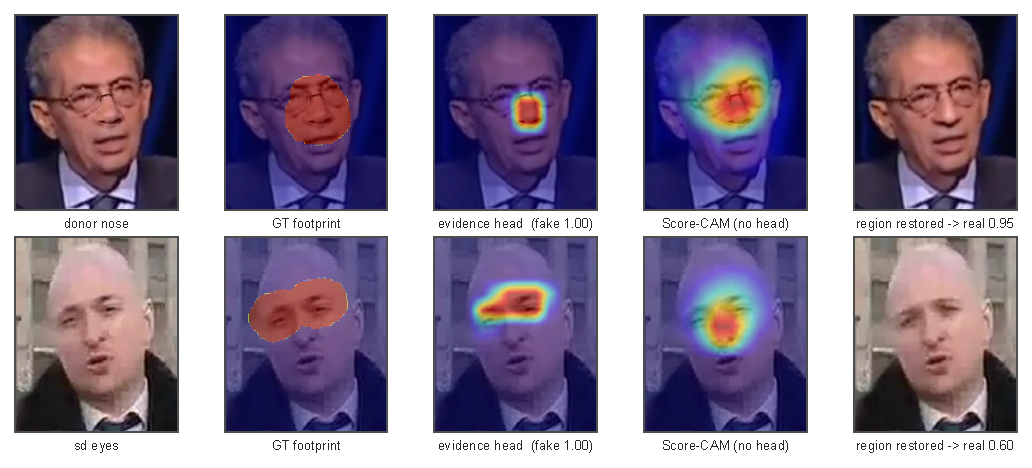
\includegraphics[width=0.72\textwidth]{fig_evidence}
\caption{Held-out part-level forgeries: input, exact footprint, evidence map with the three-way decision, Score-CAM on the
same backbone without the head, and the result of restoring the named region to the original.}
\label{fig:evidence}
\end{figure*}
On the three held-out editors the evidence head of \ours{} reaches IoU$_7$ 0.83--0.85 with the true footprint, and
restoring the region it names removes 90.9--91.7\% of its detections, against 91.2--91.9\% when the true footprint is
restored (Table~\ref{tab:cgd_explain}, Fig.~\ref{fig:evidence}). Restoring the complement removes at most 0.5\%, a centred region 42--52\% and a
random region of equal area 11--15\%. The SDXL editor, not seen in training, gives 0.827 and 90.9\% against a ceiling of
91.2\%. \ours{}-lite reaches 0.80--0.82 and 86.9--87.8\% against 87.2--87.8\%. The named region is therefore sufficient
and necessary for the model's own decision on these forgeries. Post-hoc maps on a backbone without the head do only
moderately better than a centred region (IoU$_7$ 0.26--0.41 and flips of 45--57\%, against 0.25--0.31 and 39--41\%). The footprint supervision carries the result: the same CLIP model
trained without part-level forgeries reaches 0.38--0.48 and 54--79\%, and an EfficientNet-B4 model trained on FF++ with
part-level forgeries but without the retouching data already reaches 0.72--0.75 and 83--84\%. For whole-face FF++
forgeries no method finds a small sufficient region; restoring 15\% of the face removes 22--25\% of detections for every
method and a random region 14--21\%.

\subsection{Contribution of each training signal}
The supplement varies one signal at a time. The renders alone already stop the accusation of commercial retouching
(0.6\% fake) but send single operations other than smoothing to \textsc{filter} only 10--46\% of the time (balanced
66.1\%). On held-out Tencent and Megvii bases a whitening component with a lightness change near 20 is then called real
90\% of the time, because in a four-operation render the texture change alone identifies the class. The single-operation
components raise balanced accuracy to 70.9--72.7\% over two seeds. The CLIP backbone adds 0.05 frame AUC on Celeb-DF-v2
at equal data (73.4--74.6\% balanced over two seeds), and the part-level forgeries add the evidence head and 0.005--0.010 on
Celeb-DF-v2. On the CLIP backbone they also raise the share of held-out training-service originals called
\textsc{filter} from 25--28\% to 44\% and lower balanced accuracy by 3--4\,pp; on EfficientNet-B4 the share moves from
17\% to 20\%. A RepViT-M0.9 version with the renders
(4.7\,M parameters) runs in 9.7\,ms on one CPU thread as an 18\,MB TFLite file.

% ----------------------------------------------------------------------------
\section{Limitations}
For a service never seen in training, separating lightly retouched faces from their originals stays at 70--73\%
balanced accuracy for every model we trained, below our target, and \ours{} reaches its sensitivity by sending 42\% of that
service's originals to \textsc{filter}. Per-operation recall is below the published cross-vendor numbers for eye
enlargement and lifting, and edit magnitudes could not be estimated. The test service applies one operation per image,
so combined retouching is only tested on the training services. App filters are tested through four Celeb-DF-B presets,
and \ours{}-lite accuses 40\% of untreated Celeb-DF-B genuine frames. The evidence head localises part-level forgeries
and filters, not whole-face swaps. Our reproduction of the SBI recipe reached 0.735 on Celeb-DF-v2 against 0.817 for the
released weights, so every SBI comparison uses the released checkpoint. \ours{} and \ours{}-lite are single training
runs; two seeds of the CLIP model without part-level forgeries agree within 0.005 AUC.

\section{Conclusion}
Beautification puts binary face-forgery detectors in a trade-off that no threshold resolves: on a paired corpus and on
Celeb-DF-B, each of thirteen published detectors either accuses beautified genuine faces or lets beautified deepfakes
through. A filter class removes the trade-off when it is trained with real forgeries, with degradation shared by all
classes and with commercial renders split into single operations. A CLIP-based detector trained this way matches the
strongest published detectors on cross-dataset forgery detection, is not measurably affected by beautification, and
names the regions of part-level forgeries its decision depends on. Recognising light retouching from an unseen service is the part
that remains open.

\bibliographystyle{IEEEtran}
\bibliography{refs}
\end{document}
